
\subsection{ライブラリ}
\begin{table*}[ht]
	\centering
	\scalebox{0.7}{
		\begin{tabular}{|c|c|c|c|c|c|c|c|c|c|c|c|c|c|} % Change 'l' to 'c' for center alignment
			\hline
			              & 関数名                                                    & \multicolumn{4}{c|}{センサ情報}   & \multicolumn{4}{c|}{環境情報}    & \multicolumn{4}{c|}{その他}                                                                                                                                                                                                                                                                                                                             \\ \hline
			              &                                                        &                              &                              &                              & \multicolumn{1}{c|}{BLEビーコン} &                              & \makecell{磁気                                                                                                } & \multicolumn{2}{c|}{BLEビーコン} & \multicolumn{2}{c|}{正解初期}    & \multicolumn{2}{c|}{正解補正}                                                 \\ \cline{6-6} \cline{8-8} \cline{9-9} \cline{10-10}\cline{11-12}\cline{13-14}
			              &                                                        & 加速度                          & 角速度                          & 角度                           & 電波強度                         & フロアマップ                       & FP                                                                                                            & 基地局位置                        & FP                           & 座標                               & 方向 & 座標                           & 方向 \\ \hline
			基本PDR         & estimate\_trajectory                                   & \multicolumn{1}{c|}{$\circ$} & \multicolumn{1}{c|}{$\circ$} &                              &                              &                              &                                                                                                               &                              &                              & \multicolumn{1}{c|}{$\triangle$} &    &                              &    \\ \hline
			角速度から角度推定     & convert\_to\_angle\_from\_gyro                         &                              & \multicolumn{1}{c|}{$\circ$} &                              &                              &                              &                                                                                                               &                              &                              &                                  &    &                              &    \\ \hline
			ドリフト補正        & remove\_drift\_in\_angle                               & \multicolumn{1}{c|}{$\circ$} &                              & \multicolumn{1}{c|}{$\circ$} &                              &                              &                                                                                                               &                              &                              & \multicolumn{1}{c|}{$\circ$}     &    & \multicolumn{1}{c|}{$\circ$} &    \\ \hline
			初期方向補正 フロアマップ & rotate\_trajectory\_to\_optimal\_alignment\_using\_map & \multicolumn{1}{c|}{$\circ$} &                              & \multicolumn{1}{c|}{$\circ$} &                              & \multicolumn{1}{c|}{$\circ$} &                                                                                                               &                              &                              & \multicolumn{1}{c|}{$\triangle$} &    &                              &    \\ \hline
			初期方向補正 BLE    & rotate\_trajectory\_to\_optimal\_alignment\_using\_ble & \multicolumn{1}{c|}{$\circ$} & \multicolumn{1}{c|}{$\circ$} &                              & \multicolumn{1}{c|}{$\circ$} &                              &                                                                                                               & \multicolumn{1}{c|}{$\circ$} &                              & \multicolumn{1}{c|}{$\triangle$} &    &                              &    \\ \hline
			マップマッチング補正    & move\_unwalkable\_points\_to\_walkable                 & \multicolumn{1}{c|}{$\circ$} & \multicolumn{1}{c|}{$\circ$} &                              &                              & \multicolumn{1}{c|}{$\circ$} &                                                                                                               &                              &                              &                                  &    &                              &    \\ \hline
			安定歩行区間補正      &                                                        & \multicolumn{1}{c|}{$\circ$} & \multicolumn{1}{c|}{$\circ$} &                              &                              &                              &                                                                                                               &                              &                              &                                  &    &                              &    \\ \hline
			初期方向補正 BLE FP &                                                        & \multicolumn{1}{c|}{$\circ$} & \multicolumn{1}{c|}{$\circ$} &                              &                              &                              &                                                                                                               &                              & \multicolumn{1}{c|}{$\circ$} &                                  &    &                              &    \\ \hline
		\end{tabular}
	}
	\caption{関数に必要な情報とその対応表} \label{}
	\textit{注: $\circ$は必須引数,$\triangle$はオプショナル引数を示す} \label{tab:my_label}
\end{table*}


関数に必要な引数の情報とその対応表を表1に示す.
詳しい関数の説明や内部実装については後述する.
引数の情報は大きく分けてセンサ情報,環境情報,その他の3つに分けられる.
センサ情報はスマートフォンから得られる加速度,角速度,磁気センサ,BLEビーコンの電波情報などが含まれる.
環境情報はフロアマップ情報,フロアマップにおける各BLEビーコンの配置情報などが含まれる.
これらの環境情報は全てセンサデータが与えられる前に得られる情報である.
その他はセンシング中,またはセンシング前に得られる情報であり,初期位置,終了位置などの情報が該当する.


\begin{table}[h]
	\centering
	\begin{tabular}{lll}
		\toprule
		カラム名 & 単位        & データ型  \\
		\midrule
		ts   & s (秒)     & float \\
		x    & m/s\(^2\) & float \\
		y    & m/s\(^2\) & float \\
		z    & m/s\(^2\) & float \\
		\bottomrule
	\end{tabular}
	\caption{加速度 DF}
\end{table}

\begin{table}[h]
	\centering
	\begin{tabular}{lll}
		\toprule
		カラム名 & 単位             & データ型  \\
		\midrule
		ts   & s (秒)          & float \\
		x    & rad/s (ラジアン/秒) & float \\
		y    & rad/s (ラジアン/秒) & float \\
		z    & rad/s (ラジアン/秒) & float \\
		\bottomrule
	\end{tabular}
	\caption{角速度 DF}
\end{table}


\begin{table}[ht]
	\centering
	\label{tab:first-coord-dict}
	\begin{tabular}{lll}
		\hline
		      & {データ型}         & {説明}          \\ \hline
		key   & \texttt{str}   & xまたはy         \\ \hline
		value & \texttt{float} & \makecell{座標} \\ \hline
	\end{tabular}
	\caption{正解初期座標 DICT}
\end{table}




\begin{table}[h]
	\centering
	\begin{tabular}{lll}
		\toprule
		カラム名 & 単位      & データ型  \\
		\midrule
		ts   & s (秒)   & float \\
		x    & m(メートル) & float \\
		y    & m(メートル) & float \\
		\bottomrule
	\end{tabular}
	\caption{座標DF}
\end{table}


\begin{table}[h]
	\centering
	\begin{tabular}{lll}
		\toprule
		カラム名 & 単位         & データ型  \\
		\midrule
		ts   & s (秒)      & float \\
		x    & rad (ラジアン) & float \\
		y    & rad (ラジアン) & float \\
		z    & rad (ラジアン) & float \\
		\bottomrule
	\end{tabular}
	\caption{角度 DF}
\end{table}




説明する関数の引数に必要な情報は全て表1と紐づいている.
言語にはPythonを使用した.Pythonはデータ解析や機械学習などの分野で広く使われており,
ライブラリを使用するユーザーにとっても比較的扱いやすい利点がある.
まず基本的なPDRの処理を行う関数をListing\ref{lst:pdr-trajectory}に示す.
この関数では加速度データフレーム(以下,DF),角速度DFを使用して位置推定を行う.
加速度DF,角速度DFのデータフレームのカラム名とデータ型を表2,表3に示す.
オプショナル引数として正解初期座標(ground\_truth\_first\_point)を与えられる.
正解初期座標は辞書型で表4に示す.
戻り値は時間経過に伴う2次元座標のDFと角度のDFであり,それぞれのカラム名とデータ型を表5,表6に示す.
戻り値で角度DFを返す理由として,次の補正処理をする際に角速度よりも扱いやすいためである.

歩幅の推定を行っている研究は多くある.
機会学習を用いた研究\cite{stride-length-auto-learning},
多変量解析を用いた研究\cite{stride-length-multi},
超音波センサーガジェットを用いた研究\cite{stride-length-ultrasonic}などがある.
本関数の内部処理では歩幅の値は固定値として扱っている.
本来であれば歩幅は身長,性別,年齢などの複数の要素によって動的に変化するため
固定値なのはありえず,先ほど挙げた研究のように歩幅を推定する必要がある.
しかし本ライブラリの目的は正確な歩幅を用いたPDRによる位置推定ではない.
PDRで推定した歩行軌跡を環境情報などを用いて補正を行い軌跡全体の最適化を行えるライブラリの検討である.
そのため歩幅の推定は行わず固定値として扱う.
また同様の理由で歩行タイミングの検出も正確には行わず,加速度の値が特定の閾値を超えた時に
歩行タイミングとして扱っている.
図\ref{fig:pdr}にリスト\ref{lst:pdr-trajectory}を用いてPDRによる位置推定を行った結果を示す.
LiDARで取得した座標をもとに出力された軌跡を図\ref{fig:gt-trajectory}に示す.
これを本論では正解軌跡とする.
図\ref{fig:pdr}と図\ref*{fig:gt-trajectory}を比較するとPDRによる軌跡は正解軌跡と比べて大きくずれているのがわかる.
PDR特有の解決すべきものとして
軌跡そのものの形状を正解奇跡に近づける問題と絶対位置との関連付けの問題がある.
本ライブラリを用いてこれらの問題を解消し正解軌跡に近づけていく.

% 文書内
\begin{lstlisting}[caption={基本PDR}, label=lst:pdr-trajectory]
Axis2D = Literal["x", "y"]
def estimate_trajectory(
    acc_df: pd.DataFrame,
    gyro_df: pd.DataFrame,
    *,
    ground_truth_first_point: dict[Axis2D, float] | None = None,
) -> tuple[pd.DataFrame, pd.DataFrame]:
\end{lstlisting}

\begin{figure}[h]
	\centering
	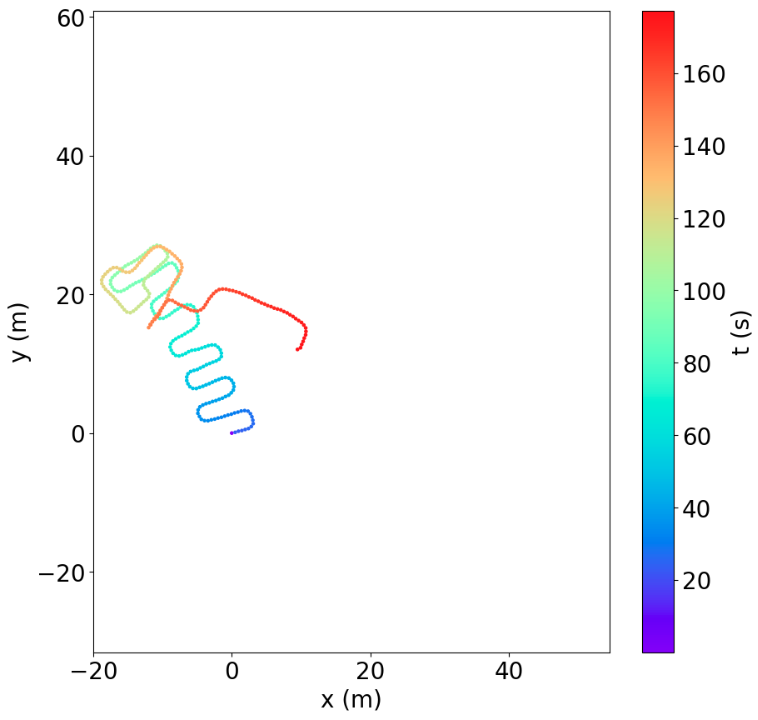
\includegraphics[width=80mm]{image/pdr.jpg}
	\caption{PDRによる軌跡}    \label{fig:pdr}
\end{figure}

Listing\ref{lst:pdr-trajectory}に示される関数に正解初期座標を
を与えたのが図\ref{fig:pdr-move}である.
予め正解座標が判明している場合はPDRによる軌跡の初期位置を補正できる.

\begin{figure}[h]
	\centering
	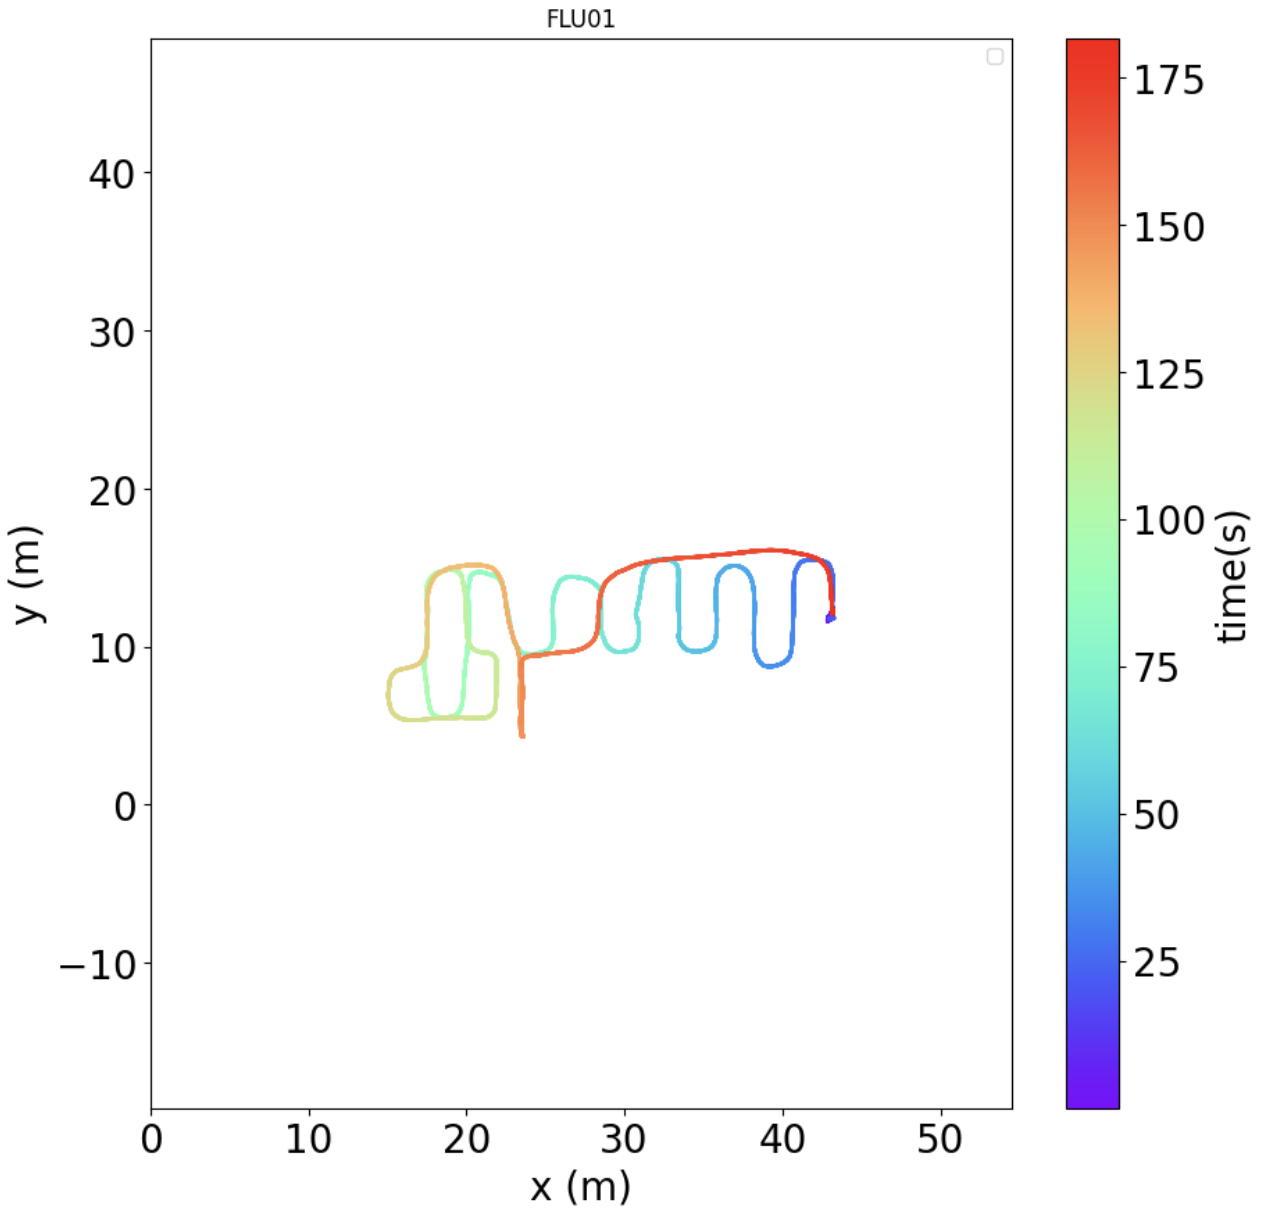
\includegraphics[width=80mm]{image/gt2.jpg}
	\caption{正解軌跡}    \label{fig:gt-trajectory}
\end{figure}

\begin{figure}[h]
	\centering
	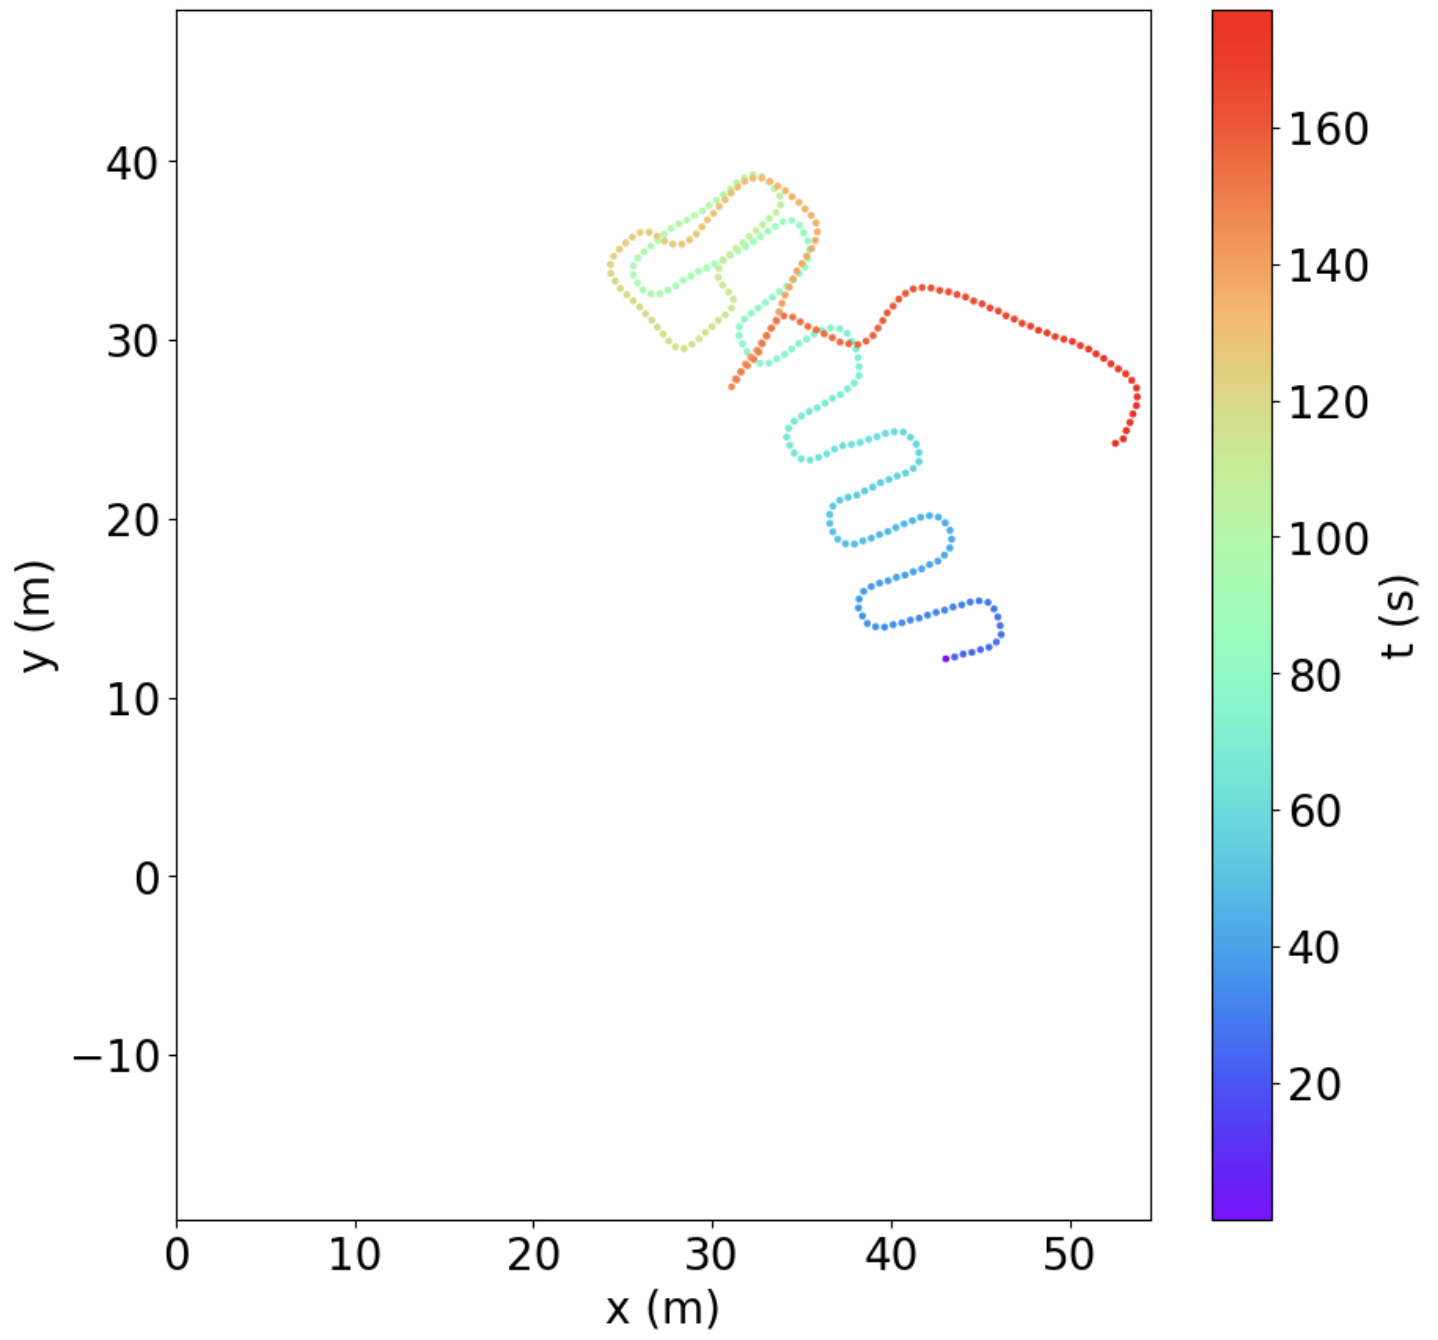
\includegraphics[width=80mm]{image/pdr-move.jpg}
	\caption{正解初期座標が存在}    \label{fig:pdr-move}
\end{figure}


図\ref{fig:pdr-move}の軌跡にはPDR特有のドリフト現象が見られる.
PDRでは角速度から進行方向を求めてその方向を元に歩行軌跡を描く.
そのため角速度センサーにわずかなでも誤差が含まれると時間経過とともにその誤差が大きくなり軌跡の形状が本来の軌跡から外れる.
この問題を解決するには角速度データに含まれる累積誤差を取り除く必要がある.


\begin{lstlisting}[caption={ドリフト除去}, label=lst:remove-drift]
def remove_drift_in_angle_df(
    acc_df: pd.DataFrame,
    angle_df: pd.DataFrame,
    ground_truth_point_df: pd.DataFrame,
) -> tuple[pd.DataFrame, pd.DataFrame]:
\end{lstlisting}

% このアルゴリズムは,角速度データに含まれる累積誤差を取り除くことで,PDRに基づく軌跡の精度を向上させる。
ドリフトを取り除く関数をListing\ref{lst:remove-drift}に示す.
引数として加速度DF,角速度DF,正解座標DFを受け取る
戻り値は時間経過に伴う2次元座標のDFと角度のDFを返す.
ドリフト補正のプロセスは,ドリフトの値を動的に計算し,それを各時刻の角度データから差し引く.
このドリフト補正プロセスは,式(1)で表される.
$\theta'(t)$は時間$t$における補正後の角度,$\theta(t)$は補正前の角度,
$\mathrm{d}$はドリフトの大きさを意味する.
この式は,時間経過に伴うドリフトの累積効果を補正するために使用される.

\vspace{5mm} % 5mmの空白を追加。必要に応じて値を調整してください。

\begin{equation}
	\theta'(t) = \theta(t) - (\mathrm{d} \times (t))
\end{equation}

\vspace{5mm} % 5mmの空白を追加。必要に応じて値を調整してください。

補正の効果を評価し適切なドリフトを見つけるために,ユークリッド距離を用いて,2つの正解座標の差異を計算する.
式(2)は,正解座標$(x_{\mathrm{n}}, y_{\mathrm{n}})$と正解座標$(x_{\mathrm{n+1}}, y_{\mathrm{n+1}})$との間のユークリッド距離$\mathrm{E}$を示している.
この式に基づきドリフト値に対してグリッドサーチを行い距離が最小になるドリフト値を探す.
最小のドリフト値を角度DFから引きそれに基づいた座標DFと角度DFを返す.
図\ref{fig:pdr-remove-drift}に示すように,ドリフト補正後の軌跡は,元の軌跡と比較して正解軌跡の形状に近づいている.
このアルゴリズムでは正解座標$(x_{\mathrm{n}}, y_{\mathrm{n}})$と正解座標$(x_{\mathrm{n+1}}, y_{\mathrm{n+1}})$の距離が近い時に特に有効である.
この処理は$(x_{\mathrm{n+2}}, y_{\mathrm{n+2}})$など2つ以上の座標が存在する場合も同様に適用できる.

\vspace{5mm} % 5mmの空白を追加。必要に応じて値を調整してください。
\begin{equation}
	\mathrm{E} = \sqrt{(x_{\mathrm{g}} - x_{\mathrm{ref}})^2 + (y_{\mathrm{g}} - y_{\mathrm{ref}})^2}
\end{equation}
\vspace{5mm} % 5mmの空白を追加。必要に応じて値を調整してください。

\begin{figure}[h]
	\centering
	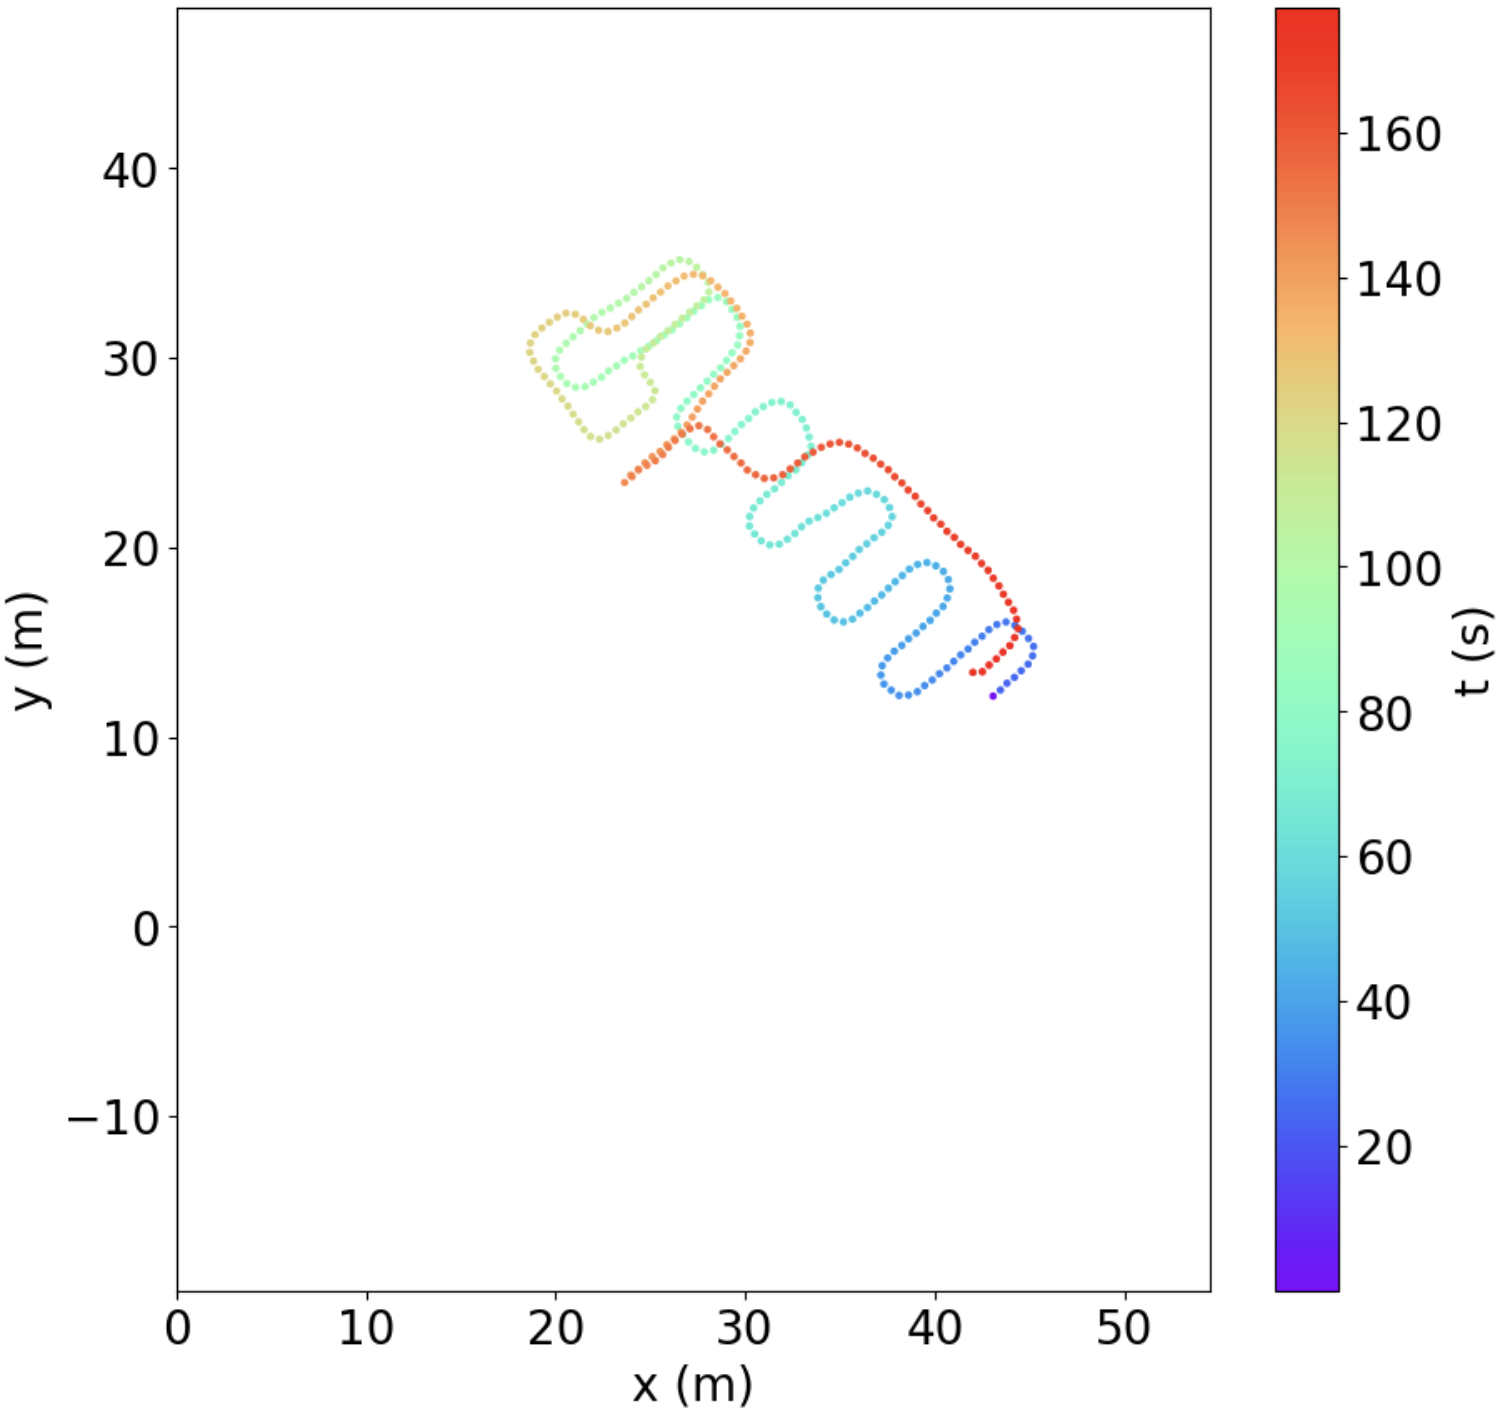
\includegraphics[width=80mm]{image/pdr-remove-drift-two.jpg}
	\caption{ドリフト補正後の軌跡}    \label{fig:pdr-remove-drift}
\end{figure}


図\ref{fig:pdr-remove-drift}の軌跡の問題点として初期方向の誤差がある.
初期方向が誤っていると,歩行者の実際の移動経路と大きく異なる軌跡になる.
この問題を解決するためには,適切な初期方向を見つけて軌跡全体を回転させる必要がある.
フロアマップ情報を元に軌跡を回転させる関数をListing\ref{lst:pdr-rotate}に示す.
引数として加速度DF,角度DF,表\ref{tab:map_dict}に示すフロアマップ情報DICT,フロア名,及びマップの1pxあたりの距離を受け取る.
内部の処理としては軌跡を回転させその時の水平垂直方向の割合を計算する.
軌跡における垂直成分と水平成分を可視化したものが図\ref{fig:color}である.
この割合が最も大きい回転角度をグリッドサーチを用いて探し最適な角度を見つける.
しかしこの処理だけでは適切な初期方向は絞り込めない.
割合が大きいものがあっても90度回転させるごとに水平垂直方向の割合が同一になるため4つの角度から適切な初期方向を見つける必要がある.
この絞り込みの処理としてマップ上の通行可能,不可能な座標の情報を利用する.
各回転角度での軌跡座標がマップ上で通行可能なポイントの数を計算し最も多いポイントを持つ回転角度を選択する.
この処理を適用した結果が図\ref{fig:pdr-rotate}である.
補正前と比べて軌跡の初期方向が正解軌跡に近づいている.

\begin{lstlisting}[caption={初期方向補正}, label=lst:pdr-rotate]
def rotate_trajectory_to
		_optimal_alignment_using_map(
    acc_df: pd.DataFrame,
    angle_df: pd.DataFrame,
    map_dict: dict[str, np.ndarray],
    floor_name: str,
    dx: float,
    dy: float,
    *,
    ground_truth_first_point: dict[Axis2D, float] | None = None,
) -> tuple[pd.DataFrame, pd.DataFrame]:
\end{lstlisting}

\begin{table}[ht]
	\centering
	\begin{tabular}{lll}
		\hline
		      & \textbf{データ型}       & \textbf{説明}             \\ \hline
		key   & \texttt{str}        & floorの名前                \\ \hline
		value & \texttt{np.ndarray} & \makecell{フロアマップの画像データ. \\各フロアのブール値の\\NumPy配列} \\ \hline
	\end{tabular}
	\caption{フロマップ DICT}
	\label{tab:map_dict}
\end{table}

\begin{figure}[h]
	\centering
	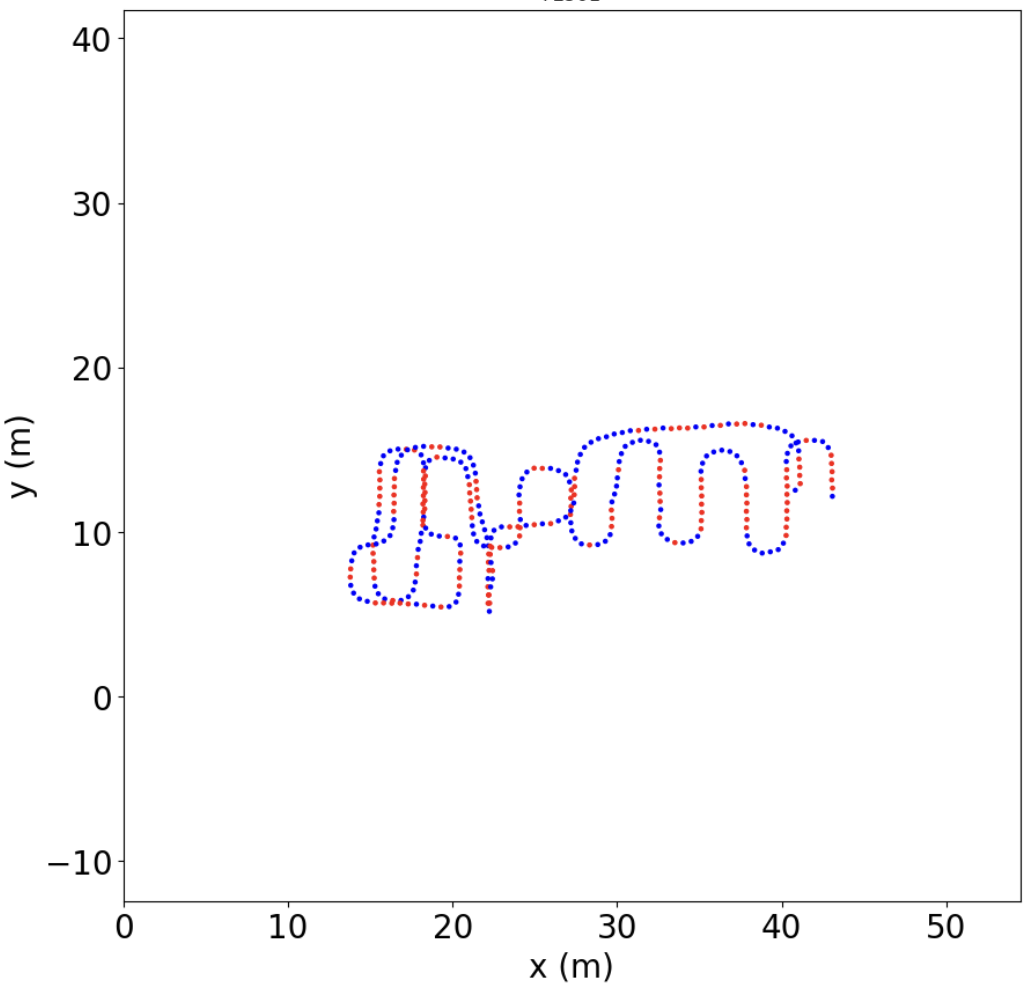
\includegraphics[width=80mm]{image/rb.jpg}
	\caption{垂直成分と水平成分の可視化}    \label{fig:color}
\end{figure}

\begin{figure}[h]
	\centering
	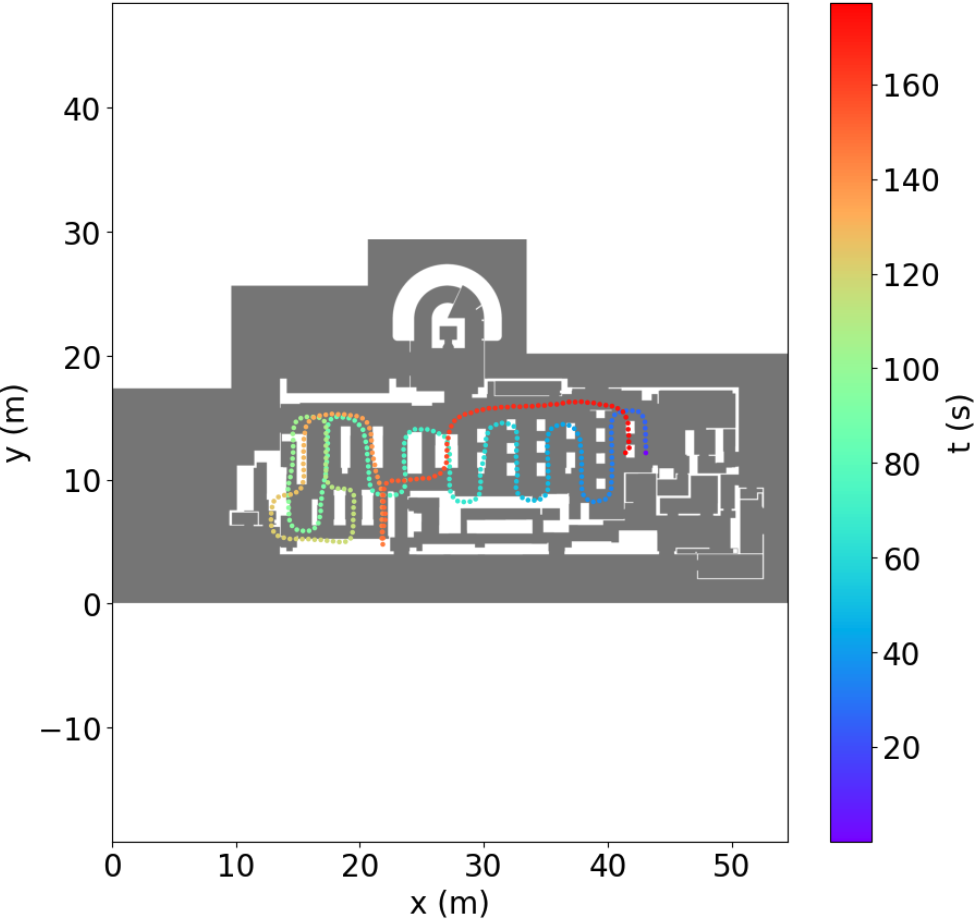
\includegraphics[width=80mm]{image/pdr-rotate.jpg}
	\caption{初期方向の補正後の軌跡}    \label{fig:pdr-rotate}
\end{figure}

フロアマップ情報を用いた初期方向補正ではマップの存在可能な点の分布によっては正しく機能しない場合がある.
別の方法としてBLEビーコンの情報を用いた初期方向補正を行う関数を提供する.
関数をListing\ref{lst:rotate-trajectory-using-ble}に示す.
この関数では加速度DF,角度DF,BLEビーコンの電波強度DF, BLEビーコンの基地局DFを受け取る.
BLEビーコンの電波強度DFとBLEビーコンの基地局DFのカラム名とデータ型を表6,表7に示す.
戻り値は時間経過に伴う2次元座標のDFと角度のDFを返す.
一定の強いRSSIの電波を受信した際の時間情報を元に時間的に近い推定軌跡の座標を取得する.
図\ref{fig:ble-merge}に示した図は時間的に近い推定軌跡の座標を時間経過に応じた色で表しており
青色の座標が配置されたBLEビーコンの座標を表している.

推定した軌跡の受信したBLEビーコンの基地局の座標との距離を計算する.
この総和が最小となるような回転角度をグリッドサーチで探し最適な角度に補正を行う.
BLEビーコンの基地局の座標との距離を計算する.

\begin{lstlisting}[caption={BLEを使用した初期方向補正}, label=lst:rotate-trajectory-using-ble]
def rotate_trajectory_to_optimal
		_alignment_using_ble(
    acc_df: pd.DataFrame,
    angle_df: pd.DataFrame,
    ble_scans_df: pd.DataFrame,
    ble_position_df: pd.DataFrame,
    *,
    ground_truth_first_point: dict[Axis2D, float] | None = None,
) -> tuple[pd.DataFrame, pd.DataFrame]:
\end{lstlisting}

\begin{figure}[h]
	\centering
	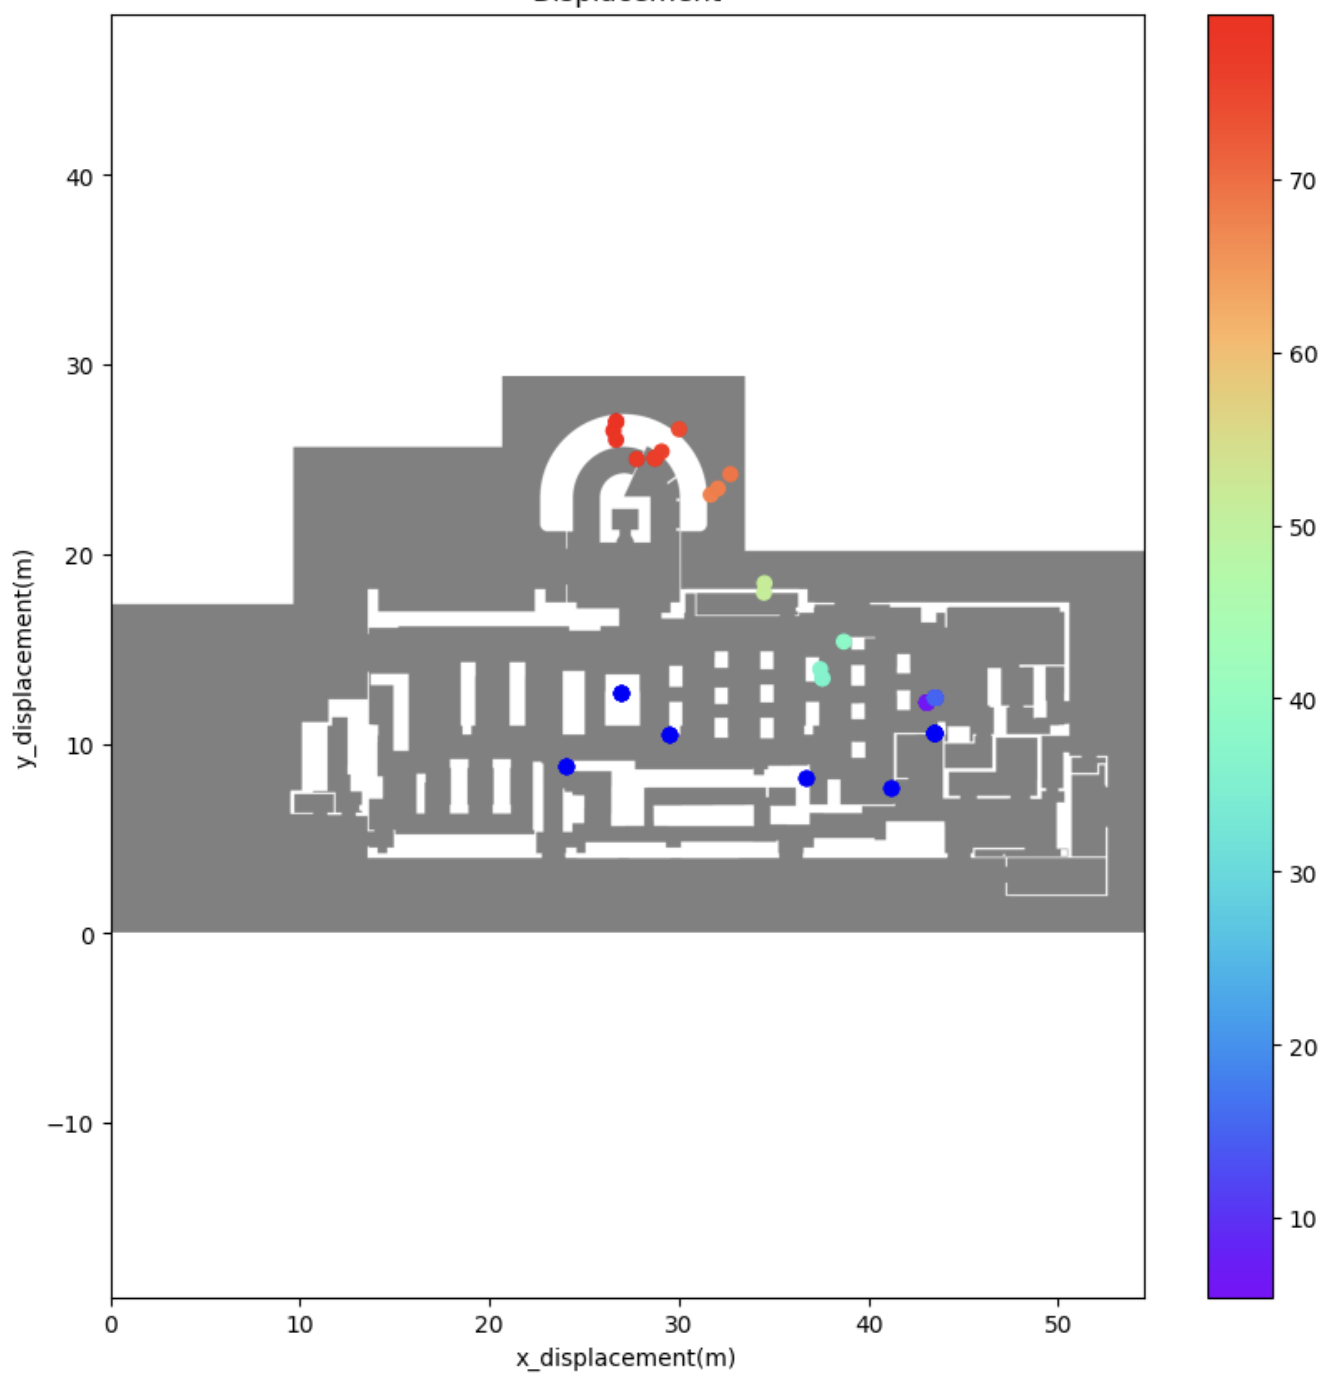
\includegraphics[width=80mm]{image/ble-merge.jpg}
	\caption{強いビーコン電波を受信した際の\\時間的に近い軌跡の座標}    \label{fig:ble-merge}
\end{figure}

\begin{table}[h]
	\centering
	\begin{tabular}{lll}
		\toprule
		カラム名      & 単位    & データ型  \\
		\midrule
		ts        & s (秒) & float \\
		bdaddress & なし    & str   \\
		rssi      & dBm   & int   \\
		\bottomrule
	\end{tabular}
	\caption{BLEビーコン電波強度DF}
\end{table}

\ref{fig:pdr-rotate}に示す軌跡の問題点として人間が歩行不可能領域を通過している点がある.
現実の人間がこのような場所を通過しないため,このような軌跡は不適切である.
そのため軌跡が歩行不可領域に存在する場合は,歩行可能な領域に移動させる処理が必要である.
この問題を解決する処理としてListing\ref{lst:map-matching}に示すマップマッチング補正関数を提供する.
マップマッチング補正関数は加速度DF,角度DF,フロアマップ情報DICT,フロア名,及びマップの1pxあたりの距離を受け取る必要がある.
戻り値は時間経過に伴う2次元座標のDFのみを返す.内部の処理の関係上補正後の角度DFは返すのが難しいためである.
関数内部ではまず加速度と角度のデータを基にして軌跡を推定する.
この軌跡に対して,各地点での座標が与えられたフロアマップ上の歩行可能な領域に存在するかどうかを検証する.
検証の結果,各地点での座標が歩行不可能な領域に存在する場合,当該座標から最も近い歩行可能な座標を幅優先探索アルゴリズムを
用いて探す.
該当する座標が見つかった場合,該当座標と該当座標以降の軌跡の座標を歩行可能な座標に平行移動して補正を行う.
当該座標の補正が終了後,次の座標に対して同様の処理を行う処理を繰り返す.
これによって軌跡の各地点が歩行可能な領域に存在するようになり,軌跡全体が最適化される.
図\ref{fig:map-matching}に示すように,マップマッチング補正後の軌跡では
歩行不可能な領域に存在していた地点がが歩行可能な地点に移動されている.

\begin{lstlisting}[caption={マップマッチング補正}, label=lst:map-matching]
def move_unwalkable_points_to_walkable(
    acc_df: pd.DataFrame,
    angle_df: pd.DataFrame,
    map_dict: dict[str, np.ndarray],
    floor_name: str,
    dx: float,
    dy: float,
    *,
    ground_truth_first_point: dict[Axis2D, float] | None = None,
) -> pd.DataFrame:

\end{lstlisting}

\begin{figure}[h]
	\centering
	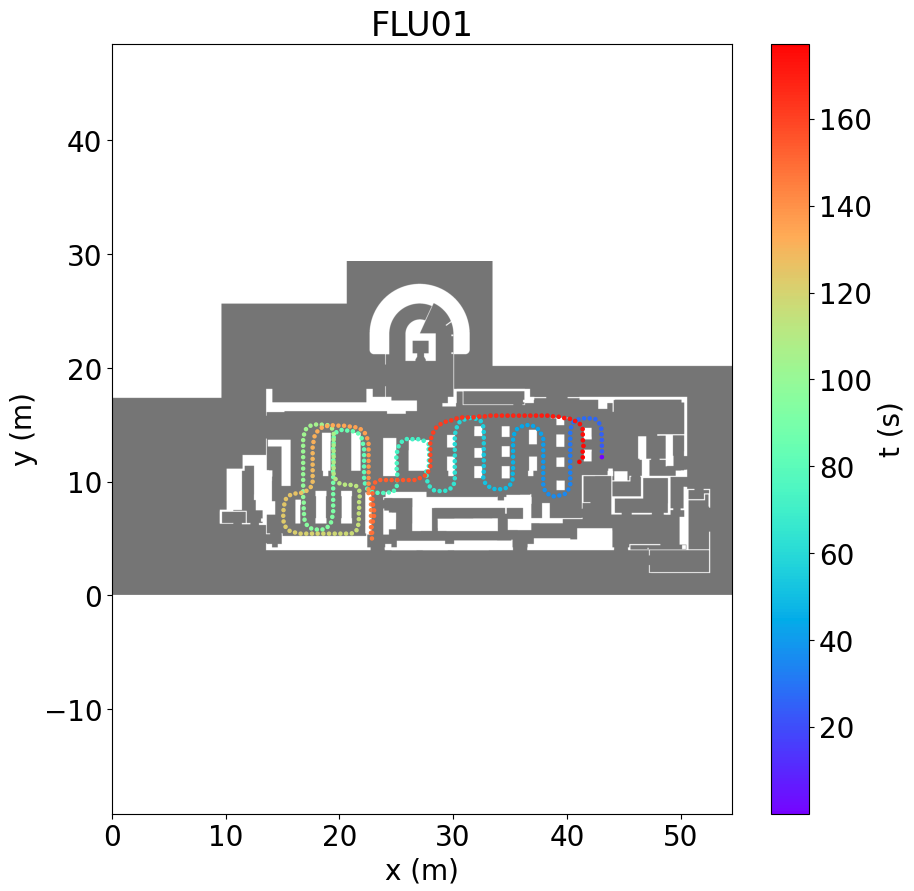
\includegraphics[width=80mm]{image/map-matching.png}
	\caption{マップマッチング補正後の軌跡}    \label{fig:map-matching}
\end{figure}


\begin{table}[h]
	\centering
	\begin{tabular}{lll}
		\toprule
		カラム名        & 単位 & データ型  \\
		\midrule
		bdaddress   & なし & str   \\
		x           & m  & float \\
		y           & m  & float \\
		floor\_name & なし & str   \\
		\bottomrule
	\end{tabular}
	\caption{BLEビーコン基地局 DF}
\end{table}
